\chapter{Symétrie particule-trou} \label{chap: ph-symmetry}

\section{Hamiltonien du modèle d'impureté d'Anderson} \label{sec:
particule-trou-h}

À demi-remplissage, le modèle d'impureté d'Anderson possède une symétrie
particule-trou qui fixe le potentiel chimique. Démontrons d'abord cette
propriété pour la partie Hubbard du hamiltonien avant d'étendre l'analyse au
couplage avec le bain. Dans le formalisme de la seconde quantification, la
transformation particule-trou prend la forme~:
\begin{align}
    c^\dagger_{i\sigma} \xrightarrow{\mathcal{P}} (-1)^i
    d_{i\bar{\sigma}}\betspace c_{i\sigma} \xrightarrow{\mathcal{P}}
    (-1)^i d^\dagger_{i\bar{\sigma}}.
    \label{eq: transformation_ph}
\end{align}
Considérons son effet une fois injecté dans le modèle de Hubbard à une bande
avec sauts aux premiers voisins~:
\begin{align}
    H_{\text{Hubbard}} = \sum_{i,j,\sigma} t_{ij}c^\dagger_{i\sigma}c_{j\sigma}
    +
    U\sum_{i}n_{i\uparrow}n_{i\downarrow} - \mu\sum_{i,\sigma}n_{i\sigma},
\end{align}
où les indices $i,j$ sont contraints aux $N$ sites du modèle. On commence par
transformer le terme cinétique en substituant les opérateurs par
\eqref{eq: transformation_ph}~:
\begin{align}
    \sum_{i,j,\sigma} t_{ij}c^\dagger_{i\sigma}c_{j\sigma}
    \xrightarrow{\mathcal{P}} \sum_{i,j,\sigma}
    t_{ij}(-1)^i d_{i\bar{\sigma}}(-1)^j d^\dagger_{j\bar{\sigma}} =
    \sum_{i,j,\sigma} t_{ij}(-1)^{i+j} d_{i\bar{\sigma}}
    d^\dagger_{j\bar{\sigma}},
\end{align}
où pour des sauts aux premiers voisins, on trouve que le coefficient vaut
toujours $(-1)^{i+j} = -1$. En utilisant l'anticommutation fermionique~:
$d_{i\bar{\sigma}} d^\dagger_{j\bar{\sigma}} = \delta_{ij} -
d^\dagger_{j\bar{\sigma}}d_{i\bar{\sigma}}$, on trouve~:
\begin{align}
    \sum_{i,j,\sigma} t_{ij}c^\dagger_{i\sigma}c_{j\sigma}
    \xrightarrow{\mathcal{P}} \sum_{i,j,\sigma}
    t_{ij}d^\dagger_{j\bar{\sigma}}d_{i\bar{\sigma}}.
\end{align}
Ensuite, grâce au changement d'indices $i \leftrightarrow j$ et, puisque les
amplitudes de sauts suivent $t_{ij} = t_{ji}$ et $t_{ii}=0$, on retrouve le
terme cinétique original sans contrainte. Pour le terme d'interaction,
l'opérateur nombre devient $n_{i\sigma} \xrightarrow{\mathcal{P}} 1 -
d^\dagger_{i\bar{\sigma}}d_{i\bar{\sigma}}$~:
\begin{align}
    U\sum_i n_{i\uparrow}n_{i\downarrow} &\xrightarrow{\mathcal{P}} U\sum_i
    (1 - d^\dagger_{i\uparrow}d_{i\uparrow})(1 -
    d^\dagger_{i\downarrow}d_{i\downarrow})
    = U\sum_i
    d^\dagger_{i\uparrow}d_{i\uparrow}d^\dagger_{i\downarrow}d_{i\downarrow}
    -U\sum_{i\sigma} d^\dagger_{i\bar{\sigma}}d_{i\bar{\sigma}} + NU.
\end{align}
La constante $NU$ peut être ignorée, car elle ne change pas la physique du
hamiltonien, mais implique seulement un décalage énergétique. Le terme de
potentiel chimique devient~:
\begin{align}
    -\mu\sum_{i,\sigma} n_{i\sigma} \xrightarrow{\mathcal{P}}
    -\mu\sum_{i,\sigma}(1 - d^\dagger_{i\bar{\sigma}}d_{i\bar{\sigma}})
    = \mu\sum_{i,\sigma} d^\dagger_{i\bar{\sigma}}d_{i\bar{\sigma}} - 2N\mu,
\end{align}
où $2N\mu$ peut aussi être ignoré pour les mêmes raisons. Le hamiltonien
transformé s'écrit donc~:
\begin{align}
    H_{\text{Hubbard}}\xrightarrow{\mathcal{P}} \sum_{i,j,\sigma}
    t_{ij}d^\dagger_{i\bar{\sigma}}d_{j\bar{\sigma}}
    +
    U\sum_{i}d^\dagger_{i\uparrow}d_{i\uparrow}d^\dagger_{i\downarrow}d_{i\downarrow}
    + (\mu - U)\sum_{i,\sigma}d^\dagger_{i\bar{\sigma}}d_{i\bar{\sigma}}.
    \label{eq: ph-hubbard}
\end{align}
Pour que la symétrie particule-trou soit parfaite, le hamiltonien doit conserver
sa forme. Comparant avec le hamiltonien original (en remplaçant $c$ par $d$),
nous devons avoir $\mu - U = -\mu$, ce qui donne~:
\begin{align}
    \boxed{\mu = \frac{U}{2}.}
    \label{eq: condition_mu_ph}
\end{align}
Cette condition garantit l'invariance du hamiltonien sous la transformation
particule-trou et que le modèle est à demi-rempli (un fermion par site).

\chapter{Article publié} \label{chap: article}

% Mémoire par articles : remplacer figs/2509.07931v2.pdf par le PDF de
% l'article publié.
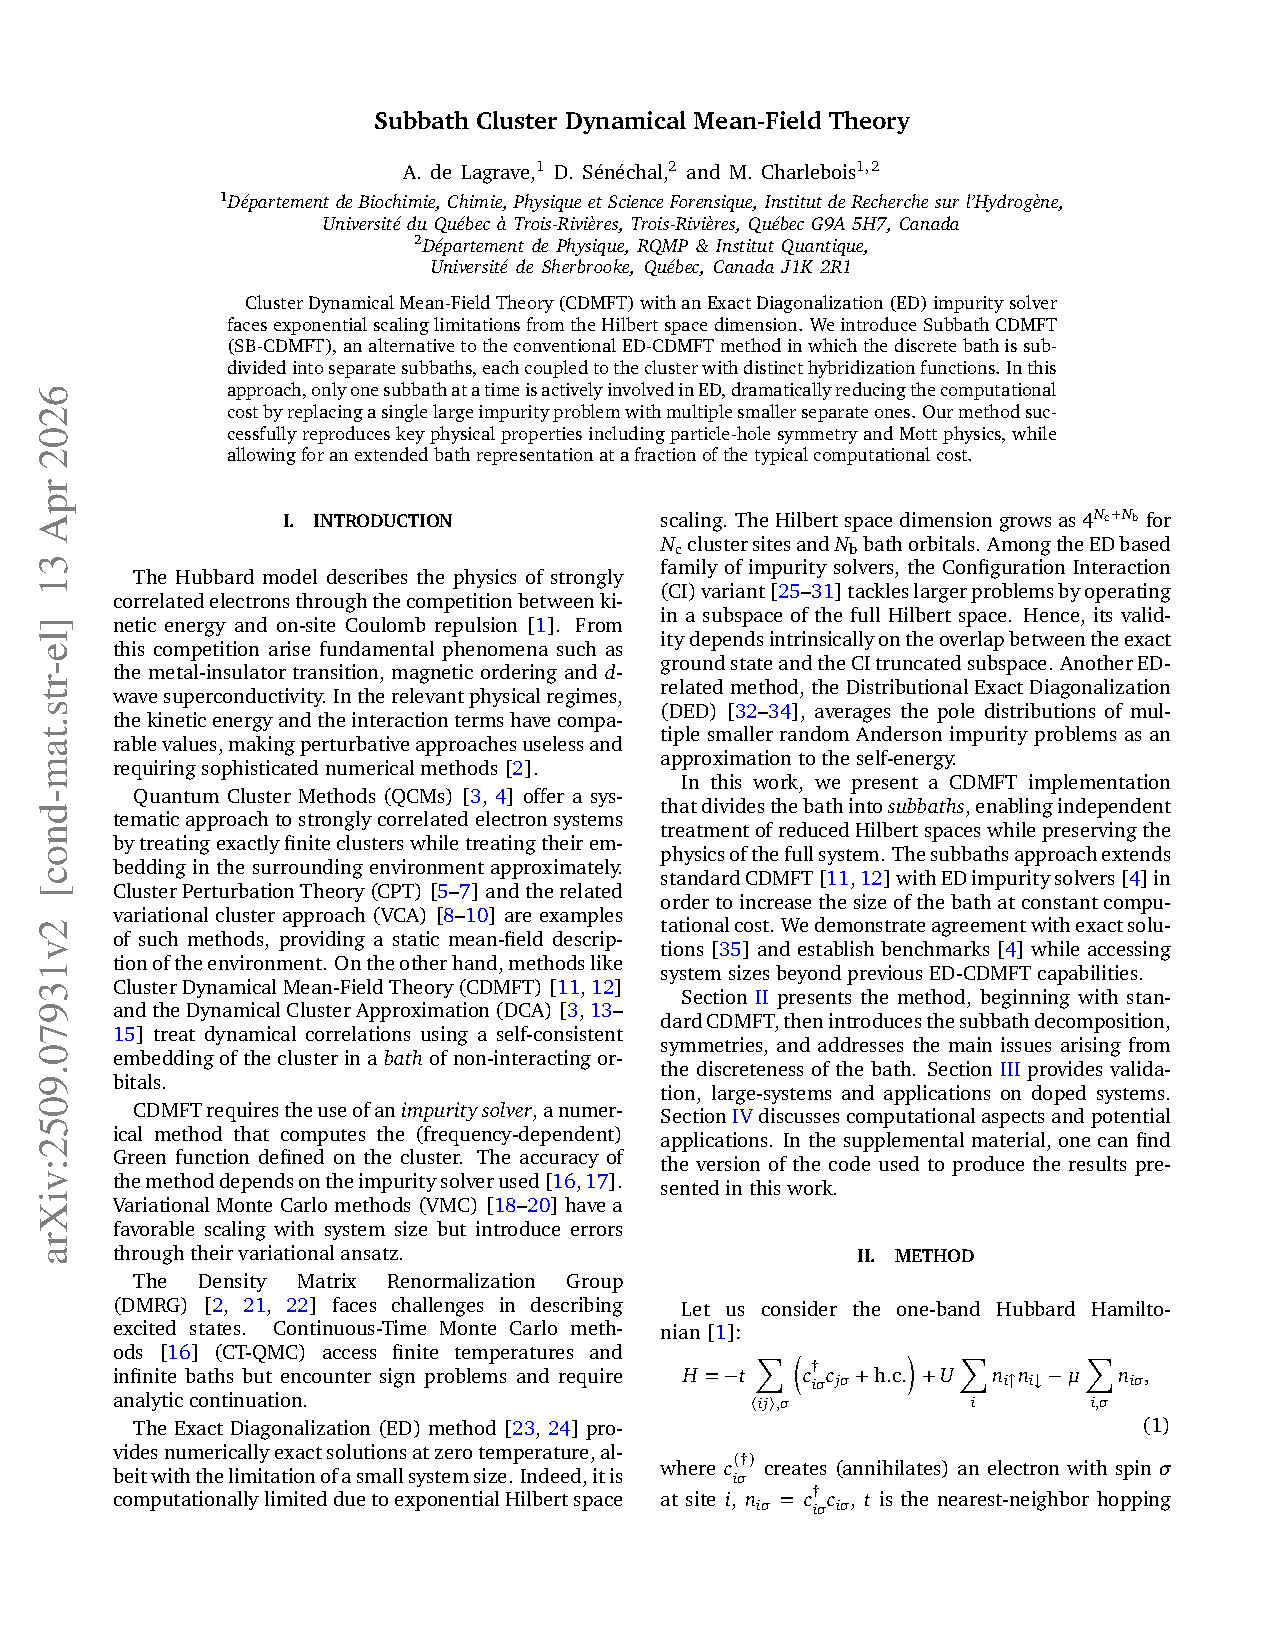
\includepdf[pages=1, fitpaper=true]{figs/2509.07931v2.pdf}
